
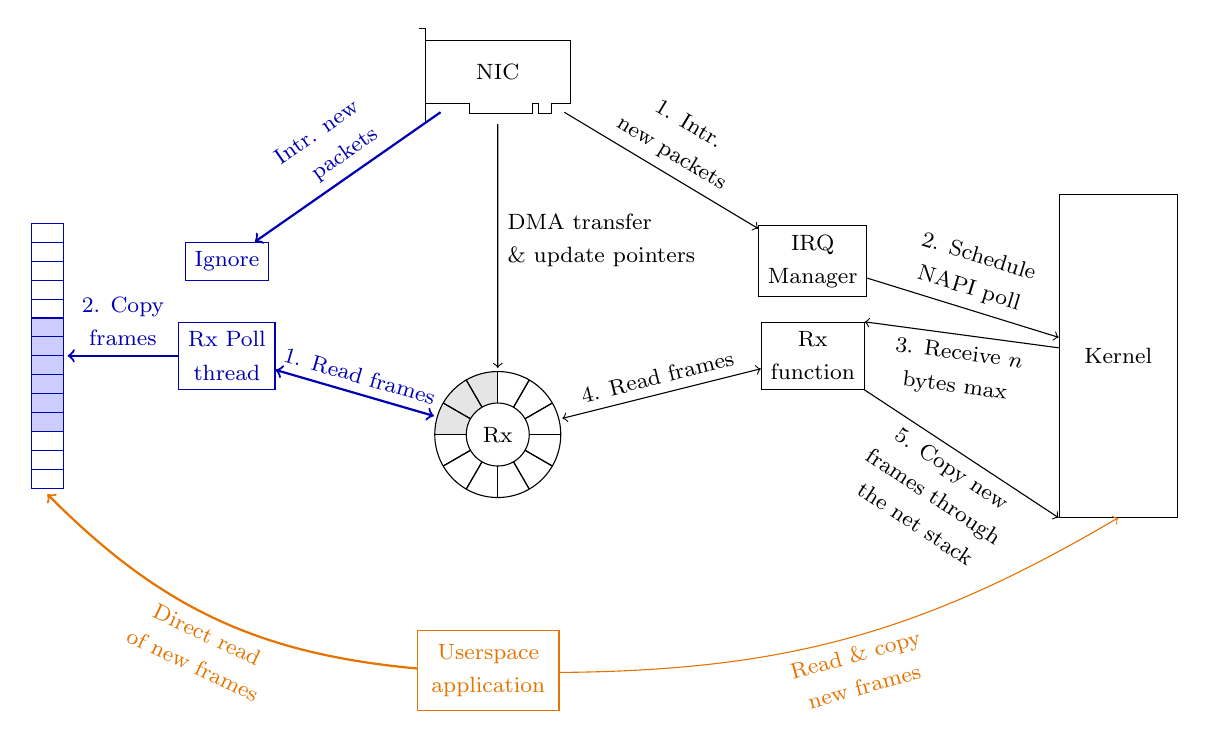
\begin{tikzpicture}[font = {\fontsize{8pt}{12}\selectfont}, scale = 0.8]
\begin{scope}[xshift = 7cm, yshift = 4cm]
\draw (-0.1, 1.2) -- (0, 1.2) -- (0,-0.3) -- (0,0) -- (0.7,0) -- (0.7,-0.15) -- (1.7, -0.15) -- (1.7, 0) -- (1.8, 0) -- (1.8, -0.15) -- (2, -0.15) -- (2,0) -- (2.3, 0) -- (2.3, 1) -- (0,1);

\node[rectangle, minimum width = 2.3cm, minimum height = 1cm] (NIC) at (1.15, 0.5) {NIC};
\end{scope}
\node[draw, align = center] (IRQ) at (13.15, 1.5) {IRQ \\ Manager};
\node[draw, minimum height = 4.1cm, minimum width = 1.5cm] (KRN) at (18, 0) {Kernel};
\node[draw, align = center] (POLL) at (13.15, 0) {Rx \\ function};

\node[draw, blue!70!black] (HIRQ) at (3.85, 1.5) {Ignore};
\node[draw, blue!70!black, align = center] (HPOLL) at (3.85, 0) {Rx Poll \\ thread};
\node[draw, orange!90!black, align = center, inner sep = 5pt] (APP) at (8, -5) {Userspace \\ application};

\begin{scope}[xshift = 8.15cm, yshift = -1.25cm, rotate = 90]
\fill[gray!20!white] (0,0) -- (0,1) arc (90:0:1cm) -- cycle;
\foreach \x in {0, 30, ..., 360}
	\draw ({cos(\x)}, {sin(\x)}) -- ({-cos(\x)}, {-sin(\x)});
\draw (0,0) circle [radius = 1cm];
\draw[black, fill = white] (0,0) circle [radius = 0.5cm]; % Poor man's \clip for intersecting regions
\node[circle, inner sep = 0.45cm] (RNG) at (0,0) {Rx};
\end{scope}

\begin{scope}[xshift = 1cm, yshift = 0cm]
\fill[blue!20!white] (-0.25, -1.2) rectangle (0.25, 0.6);
\draw[blue!70!black] (-0.25, -2.1) rectangle (0.25, 2.1);
\node[blue!70!black, rectangle, minimum width = 0.5cm, minimum height = 3.5cm] (HBUF) at (0,0) {};
\foreach \x in {-2.1, -1.8, ..., 2.1}
	\draw[blue!70!black] (-0.25, \x) -- (0.25, \x);
\end{scope}


\draw[->] (NIC) -- node[midway, above, align = center, sloped] {1. Intr. \\ new packets} (IRQ);
\draw[thick, ->, blue!70!black] (NIC) -- node[midway, above, sloped, align = right] {Intr. new \\ packets} (HIRQ);
\draw[->] (IRQ) -- node[midway, above, sloped, align = center] {2. Schedule \\ NAPI poll} (KRN);
\draw[->] (KRN) -- node[midway, below, sloped, align = center] {3. Receive $n$ \\ bytes max} (POLL.north east);
\draw[->, shorten <= 0.15cm] (NIC) -- node[midway, right, align = left] {DMA transfer \\ \& update pointers} (RNG);
\draw[<->] (POLL) -- node[midway, above, align = center, sloped] {4. Read frames} (RNG);
\draw[->] (POLL) -- node[midway, below, align = center, sloped] {5. Copy new \\ frames  through \\ the net stack} (KRN.south west);
\draw[thick, <->, blue!70!black] (RNG) -- node[midway, above, sloped] {1. Read frames} (HPOLL);
\draw[->, thick, blue!70!black] (HPOLL) -- node[midway, above, align = center] {2. Copy \\ frames} (HBUF);
\draw[->, orange!90!black, thick] (APP) to[bend left = 20] node[midway, below, sloped, align = center] {Direct read \\ of new frames} (HBUF.south);
\draw[->, orange!90!black] (APP) to[bend right = 15] node[midway, below, sloped, align = center] {Read \& copy \\ new frames} (KRN.south);
\end{tikzpicture}
